\documentclass{beamer}
\usetheme{dianahep}
%%
% The following was originally taken from a presentation by 
% Jim Pivarski (Princeton University)
% https://www.overleaf.com/7414462kswnjkcfbght#/25712329/
% with subsequent modifications here.
%

%
% Choose how your presentation looks.
%
% For more themes, color themes and font themes, see:
% http://deic.uab.es/~iblanes/beamer_gallery/index_by_theme.html
%
\mode<presentation>
{
  \usetheme{default}      % or try Darmstadt, Madrid, Warsaw, ...
  \usecolortheme{default} % or try albatross, beaver, crane, ...
  \usefonttheme{default}  % or try serif, structurebold, ...
  \setbeamertemplate{navigation symbols}{}
  \setbeamertemplate{caption}[numbered]
  \setbeamertemplate{footline}[page number]
  \setbeamercolor{frametitle}{fg=white}
  \setbeamercolor{footline}{fg=black}
} 

\usepackage[english]{babel}
\usepackage[utf8x]{inputenc}
\usepackage{tikz}
\usepackage{listings}
\usepackage{courier}

\xdefinecolor{darkblue}{rgb}{0.1,0.1,0.7}
\xdefinecolor{dianablue}{rgb}{0.18,0.24,0.31}
\definecolor{commentgreen}{rgb}{0,0.6,0}
\definecolor{stringmauve}{rgb}{0.58,0,0.82}

\lstset{ %
  backgroundcolor=\color{white},      % choose the background color
  basicstyle=\ttfamily\small,         % size of fonts used for the code
  breaklines=true,                    % automatic line breaking only at whitespace
  captionpos=b,                       % sets the caption-position to bottom
  commentstyle=\color{commentgreen},  % comment style
  escapeinside={\%*}{*)},             % if you want to add LaTeX within your code
  keywordstyle=\color{blue},          % keyword style
  stringstyle=\color{stringmauve},    % string literal style
  showstringspaces=false,
  showlines=true
}

\lstdefinelanguage{scala}{
  morekeywords={abstract,case,catch,class,def,%
    do,else,extends,false,final,finally,%
    for,if,implicit,import,match,mixin,%
    new,null,object,override,package,%
    private,protected,requires,return,sealed,%
    super,this,throw,trait,true,try,%
    type,val,var,while,with,yield},
  otherkeywords={=>,<-,<\%,<:,>:,\#,@},
  sensitive=true,
  morecomment=[l]{//},
  morecomment=[n]{/*}{*/},
  morestring=[b]",
  morestring=[b]',
  morestring=[b]"""
}



\title{LHC - Compute for Data-Driven Research Round-Table}
\author{Peter Elmer \\ Princeton University}
\date{7 Jun, 2017} 

\begin{document}

%\logo{\pgfputat{\pgfxy(0.11, 8)}{\pgfbox[right,base]{\tikz{\filldraw[fill=dianablue, draw=none] (0 cm, 0 cm) rectangle (50 cm, 1 cm);}}}\pgfputat{\pgfxy(0.11, -0.6)}{\pgfbox[right,base]{\tikz{\filldraw[fill=dianablue, draw=none] (0 cm, 0 cm) rectangle (50 cm, 1 cm);}
\includegraphics[height=0.99 cm]{images/diana-hep-logo.png}\tikz{\filldraw[fill=dianablue, draw=none] (0 cm, 0 cm) rectangle (4.9 cm, 1 cm);}}}}




\begin{frame}
  \titlepage
\end{frame}

%\logo{\pgfputat{\pgfxy(0.11, 8)}{\pgfbox[right,base]{\tikz{\filldraw[fill=dianablue, draw=none] (0 cm, 0 cm) rectangle (50 cm, 1 cm);}
\includegraphics[height=1 cm]{images/diana-hep-logo.png}}}}




% Uncomment these lines for an automatically generated outline.
%\begin{frame}{Outline}
%  \tableofcontents
%\end{frame}

\begin{frame}
\frametitle{Questions}

\begin{itemize}
\item What kind of research are you doing with data?
\item Any privacy issues with the data? Reliability?
\item What kind of data and what size/features ("by the numbers")
\item What institutions are involved in collaboration? And how do they share data?
\item Data created by the team or acquired from elsewhere?
\item What storage/compute platforms are you currently using (private, local shared, public)?
\item How is data, computation/storage, and results shared among PIs/institutions?
\item What would best accelerate your research? (tools, training, public resources)
\end{itemize}

\end{frame}



%\begin{frame}
\frametitle{Large Hadron Collider}

\begin{itemize}
\item What kind of research are you doing with data?
\item Any privacy issues with the data? Reliability?
\item What kind of data and what size/features ("by the numbers")
\item What institutions are involved in collaboration? And how do they share data?
\item Data created by the team or acquired from elsewhere?
\item What storage/compute platforms are you currently using (private, local shared, public)?
\item How is data, computation/storage, and results shared among PIs/institutions?
\item What would best accelerate your research? (tools, training, public resources)
\end{itemize}

\end{frame}



\begin{frame}
\frametitle{LHC Grand Challenge Research Questions}

The goal of HEP (and the LHC) is to understand the fundamental building blocks of nature, and their interactions. The potential of the LHC has been demonstrated in its first years with the discovery of the Higgs Boson. \\
\vskip 0.15in
\begin{figure}[htbp]
\begin{center}
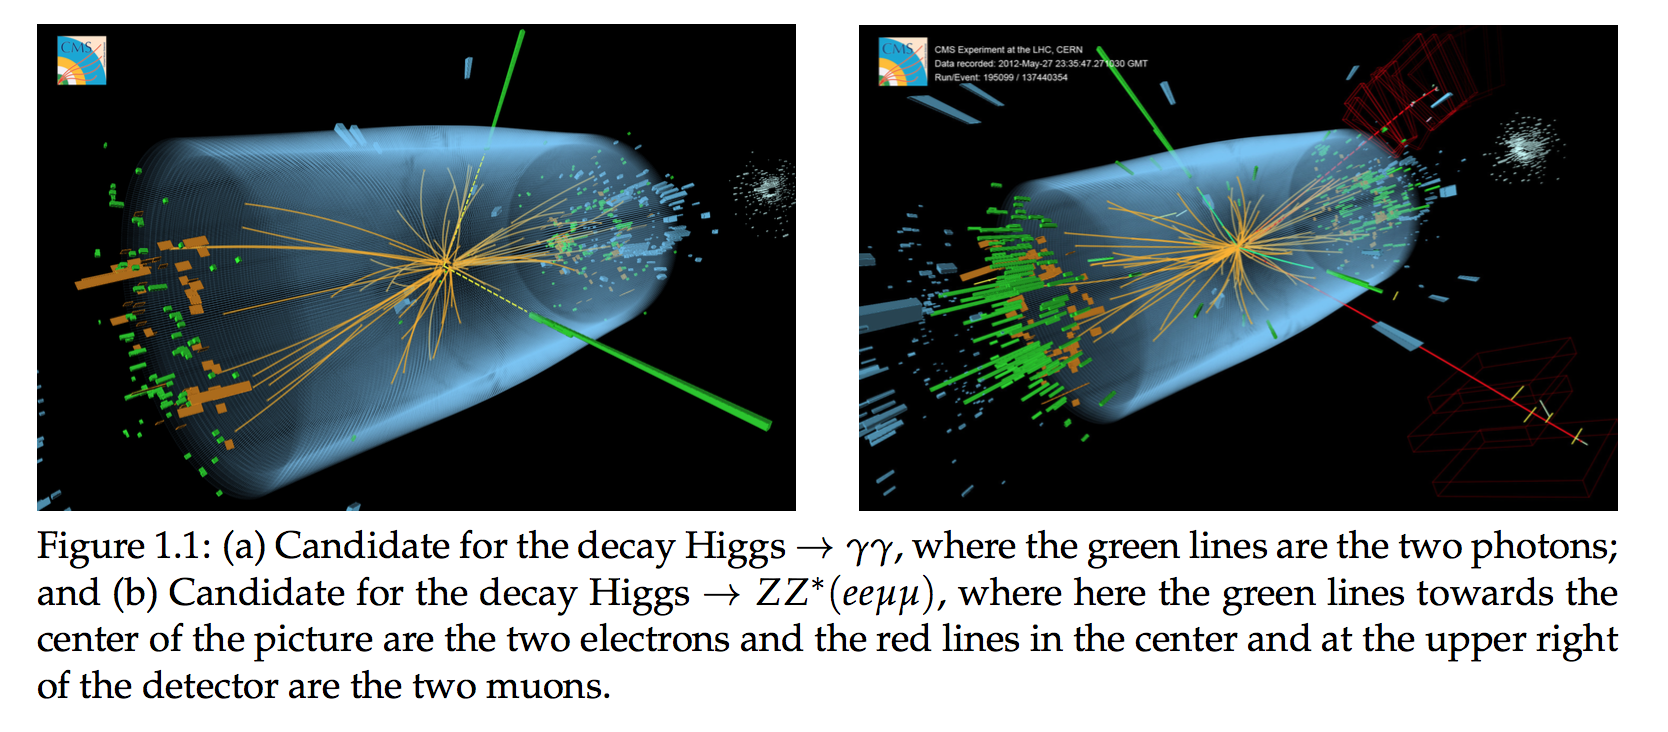
\includegraphics[width=1.0\textwidth]{images/cms-higgs-events.png}
%\caption{}
%\label{fig:example2}
\end{center}
\end{figure}

\end{frame}



\begin{frame}
\frametitle{LHC Grand Challenge Research Questions}

Many fundamental questions remain, however, including: Why does nature express the symmetries embodied in the SM, and not other equally elegant symmetries? Why are there (only) three generations of basic building blocks of matter? Why are the masses of these building blocks so different from each other, both within a generation and between generations? What is the dark matter which pervades the Universe? Why is matter so dominant over antimatter in the Universe? Does space-time have additional symmetries or extend beyond the 3+1 dimensions of which we know? What mechanism stabilizes the Higgs mass from large quantum corrections at high energy? Are neutrinos their own anti-particles? Can gravity and quantum mechanics be described in a consistent theoretical framework?

\end{frame}



\begin{frame}
\frametitle{Large Hadron Collider (LHC) and Experiments}

\begin{figure}[htbp]
\begin{center}
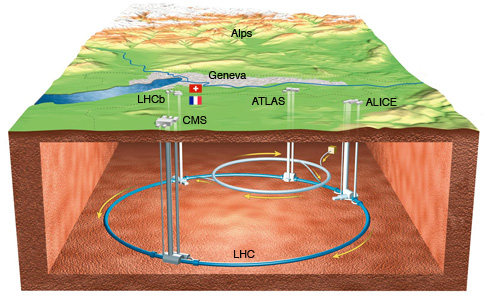
\includegraphics[width=0.8\textwidth]{images/CERNMap.jpg}
%\caption{}
%\label{fig:example2}
\end{center}
\end{figure}

\small{Two very large experiments (Atlas, CMS) with 3500+ people, and two large experiments (Alice, LHCb) with 500+ people}

\end{frame}



\begin{frame}
\frametitle{Worldwide LCG Computing Grid}

\begin{figure}[htbp]
\begin{center}
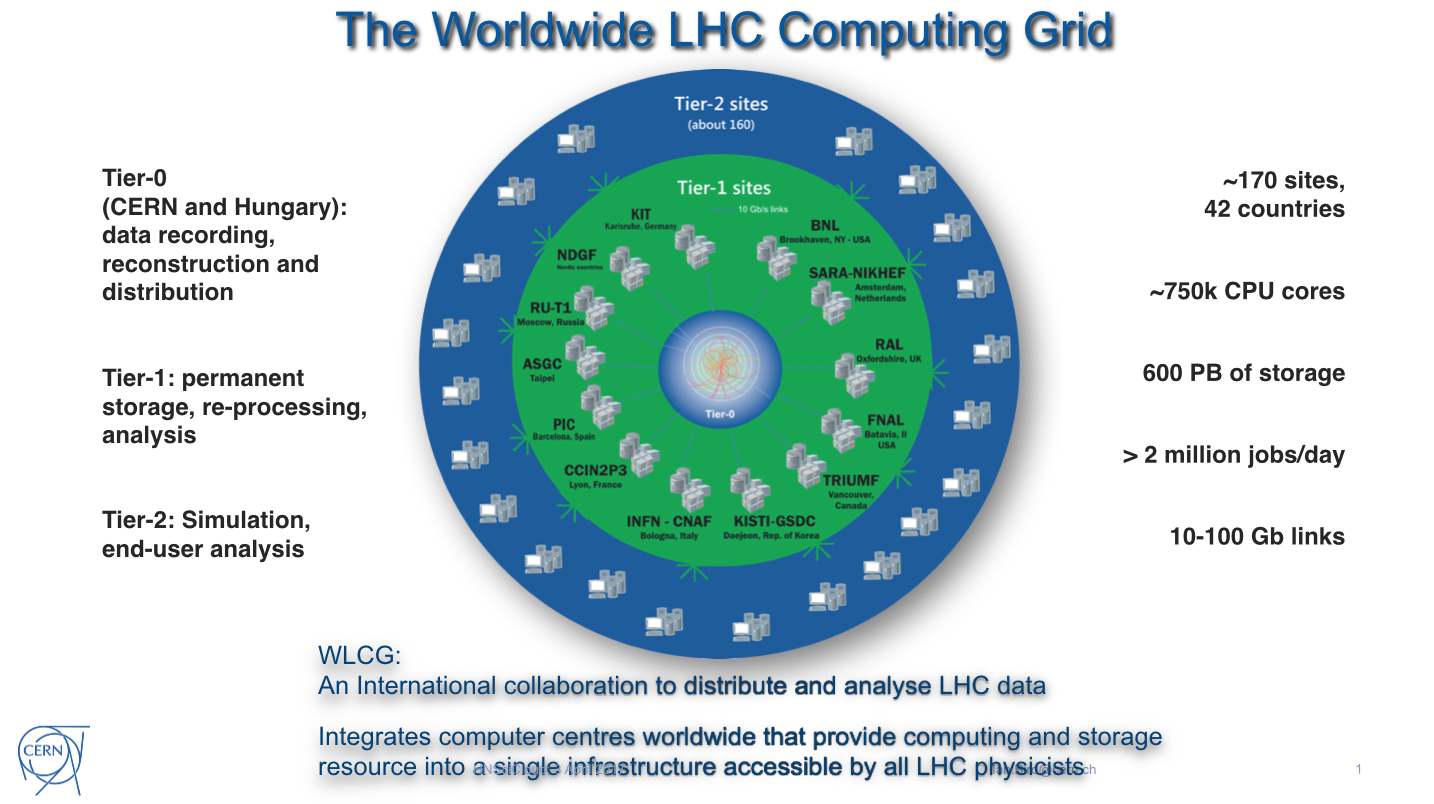
\includegraphics[width=1.0\textwidth]{images/WLCG-2017.png}
%\caption{}
%\label{fig:example2}
\end{center}
\end{figure}
\end{frame}



\begin{frame}
\frametitle{Plans for upgrading the LHC and Experiment Detectors}

\begin{figure}[htbp]
\begin{center}
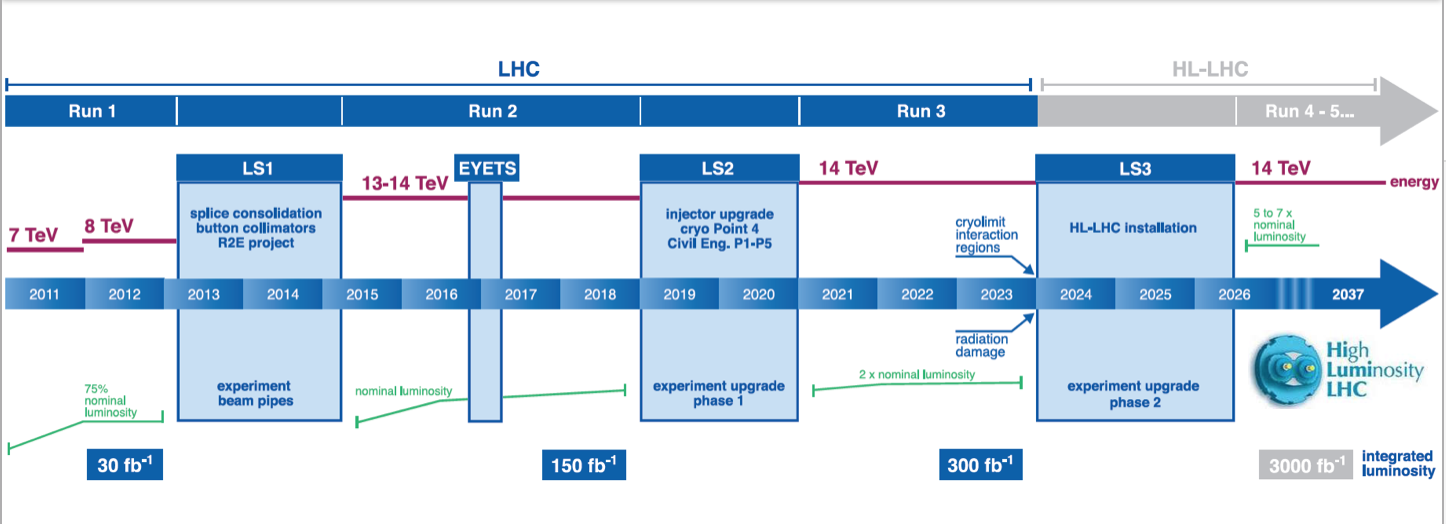
\includegraphics[width=1.0\textwidth]{images/lhc-upgrade-timeline-detail.png}
%\caption{}
%\label{fig:example2}
\end{center}
\end{figure}

\small{We estimate x60 CPU and more than x10 storage needs in 2026 for the High Luminosity LHC (HL-LHC)}

\end{frame}



\begin{frame}
\frametitle{Large Hadron Collider Notes}

\begin{itemize}
\item (Geographically) Distributed High Throughput Computing
\item Currently aggregating resources from US Universities (NSF and local
compute), DOE labs (FNAL, BNL, SLAC), and international 
\item Going forward we expect we will need to aggregate over ``owned'' resources, DOE HPC resources (e.g. NERSC, ANL, ORNL) {\it and} commercial clouds
\item FNAL HEPCloud: demonstrated at-scale use with AWS and Google Cloud 
\item TIFR Mumbai currently testing with Microsoft Azure
\item DOE (HTC on) HPC: Ongoing work to use Mira (ANL) and Edison/Cori (NERSC)
\end{itemize}

\end{frame}



\begin{frame}
\frametitle{Analysis Data Reduction - ``Last Mile''}

\begin{figure}[htbp]
\begin{center}
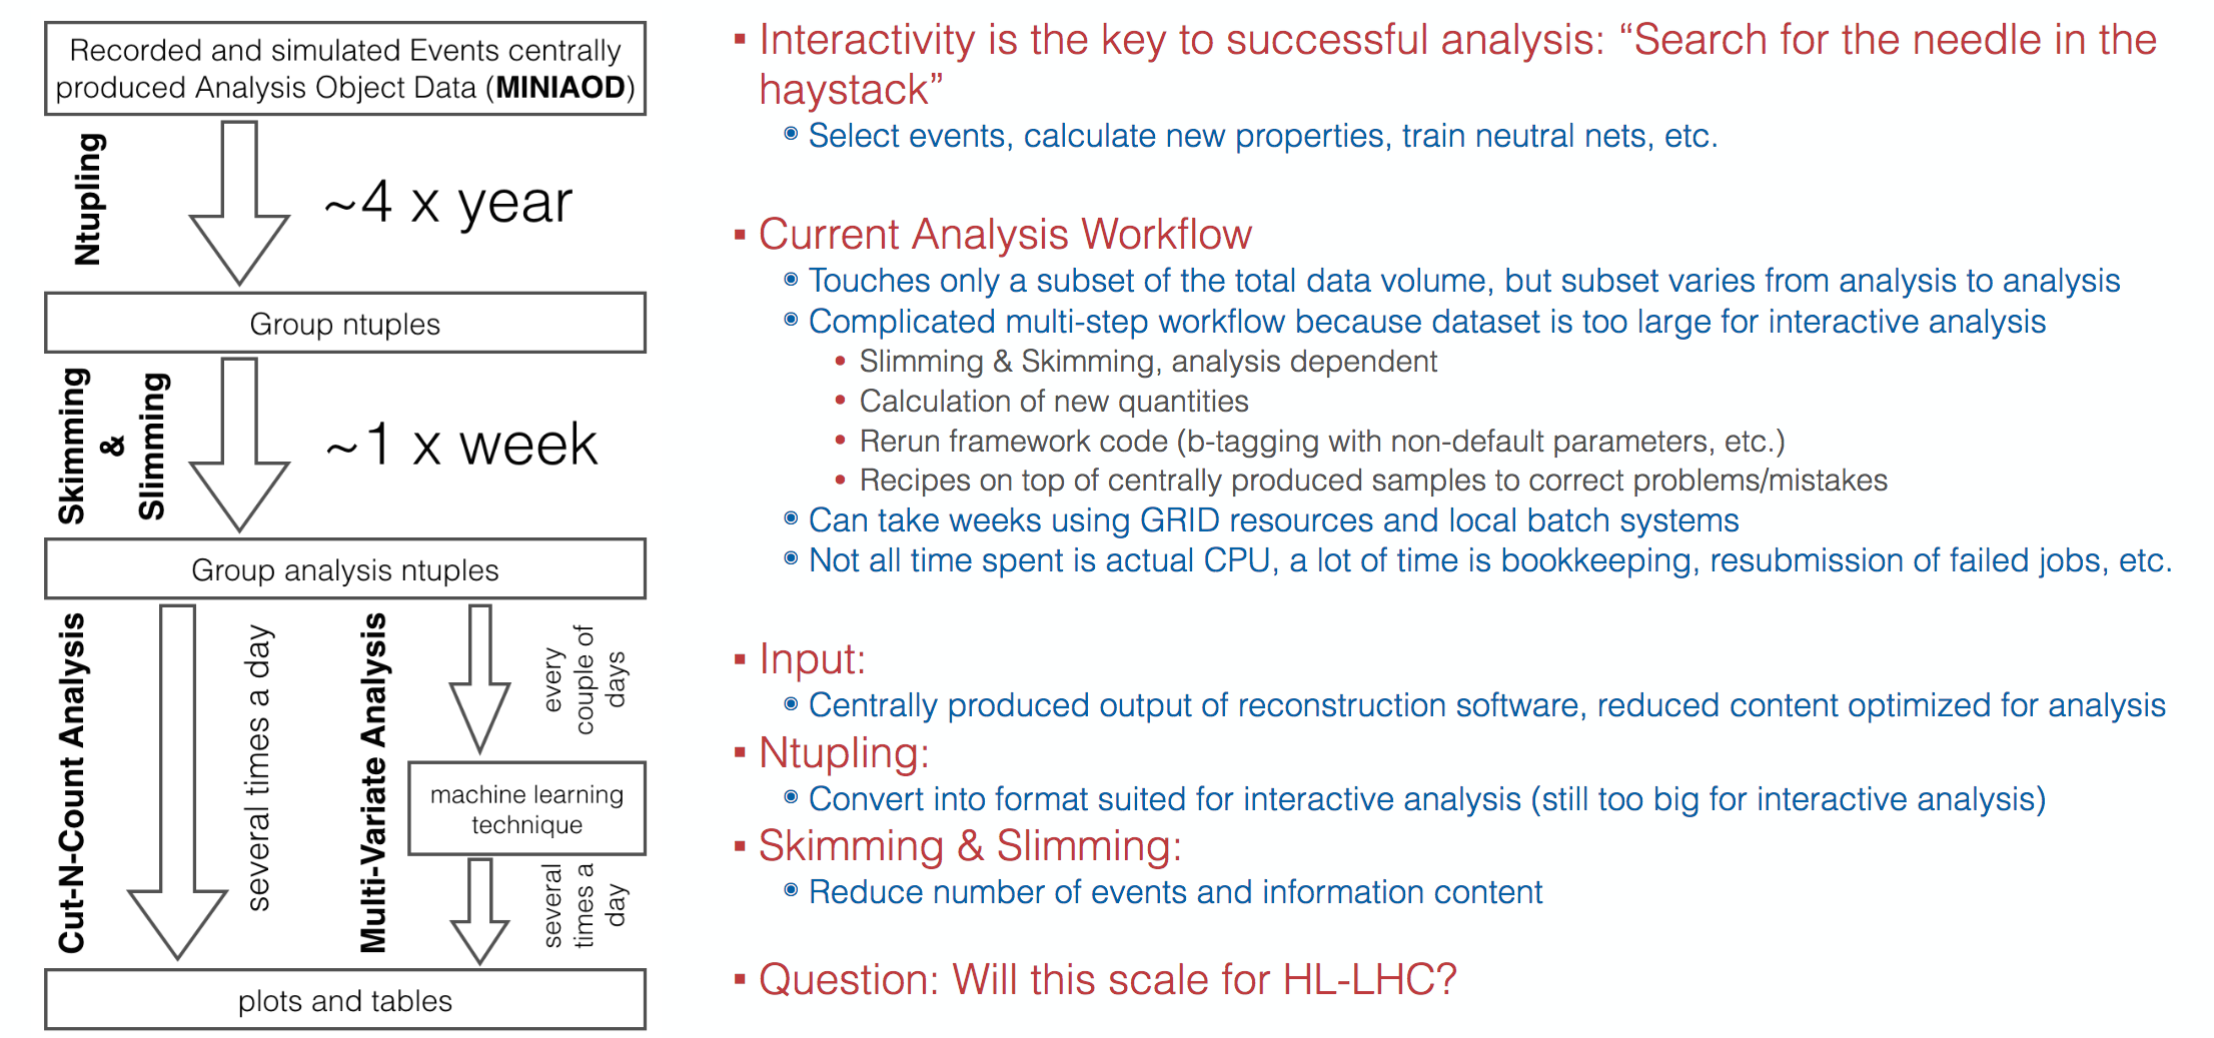
\includegraphics[width=1.0\textwidth]{images/analysis-data-reduction.png}
%\caption{}
%\label{fig:example2}
\end{center}
\end{figure}

\end{frame}



\begin{frame}
\frametitle{}

\begin{center}
    Backup slides
\end{center}

\end{frame}



\begin{frame}
\frametitle{Estimates of Resource Needs for HL-LHC (WLCG)}

\begin{figure}[htbp]
\begin{center}
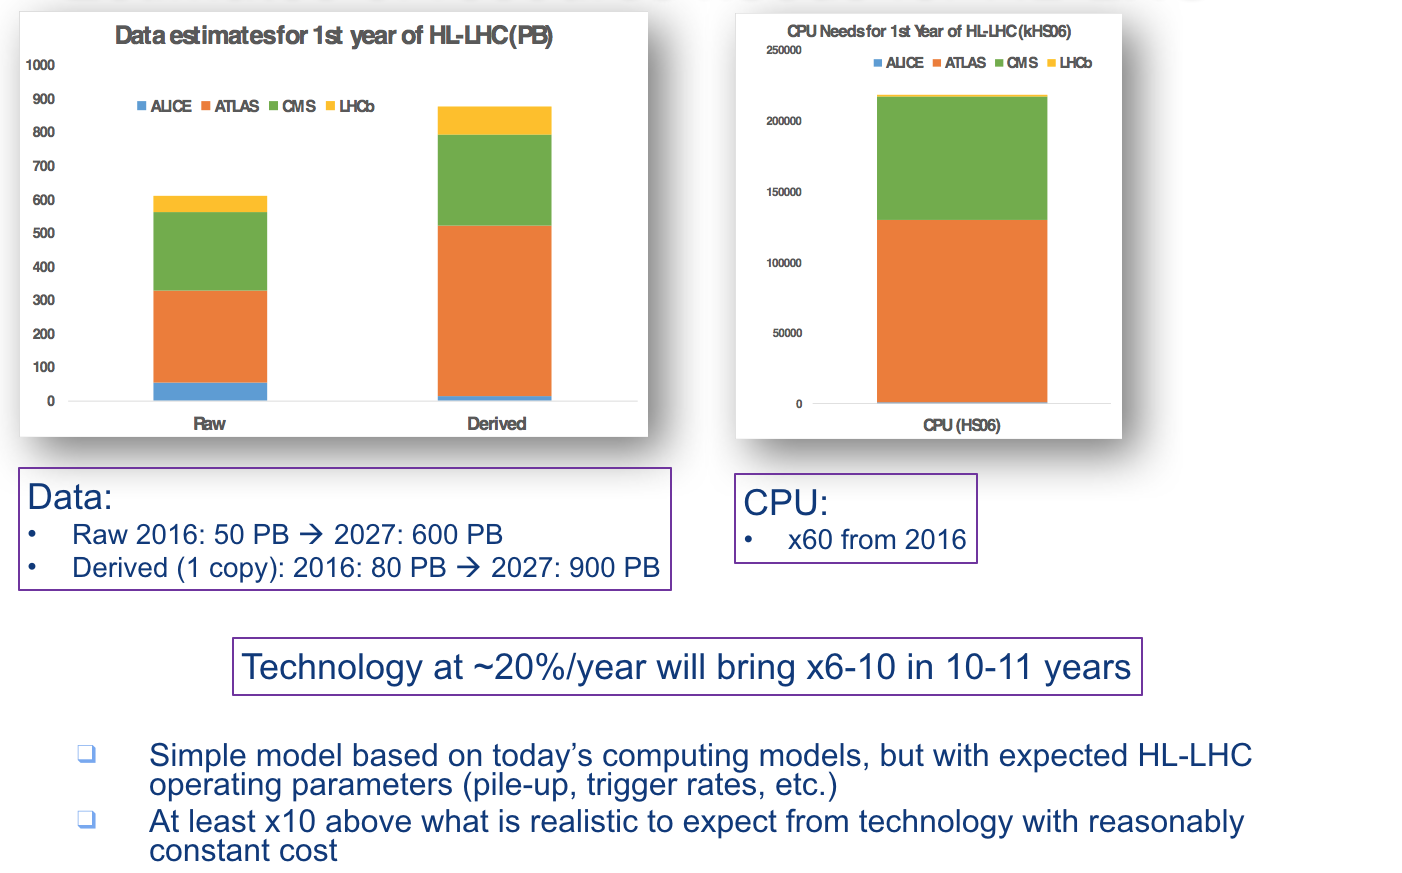
\includegraphics[width=0.95\textwidth]{images/20161008-wlcg-intro-ian-bird-slide-10.png}
\end{center}
\end{figure}

%\begin{center}
%\small{(Slide from WLCG Workshop Intro, Ian Bird, 8 Oct, 2016)}
%\end{center}

\end{frame}



\begin{frame}
\frametitle{HepCloud (Fermilab) AWS test}

\begin{figure}[htbp]
\begin{center}
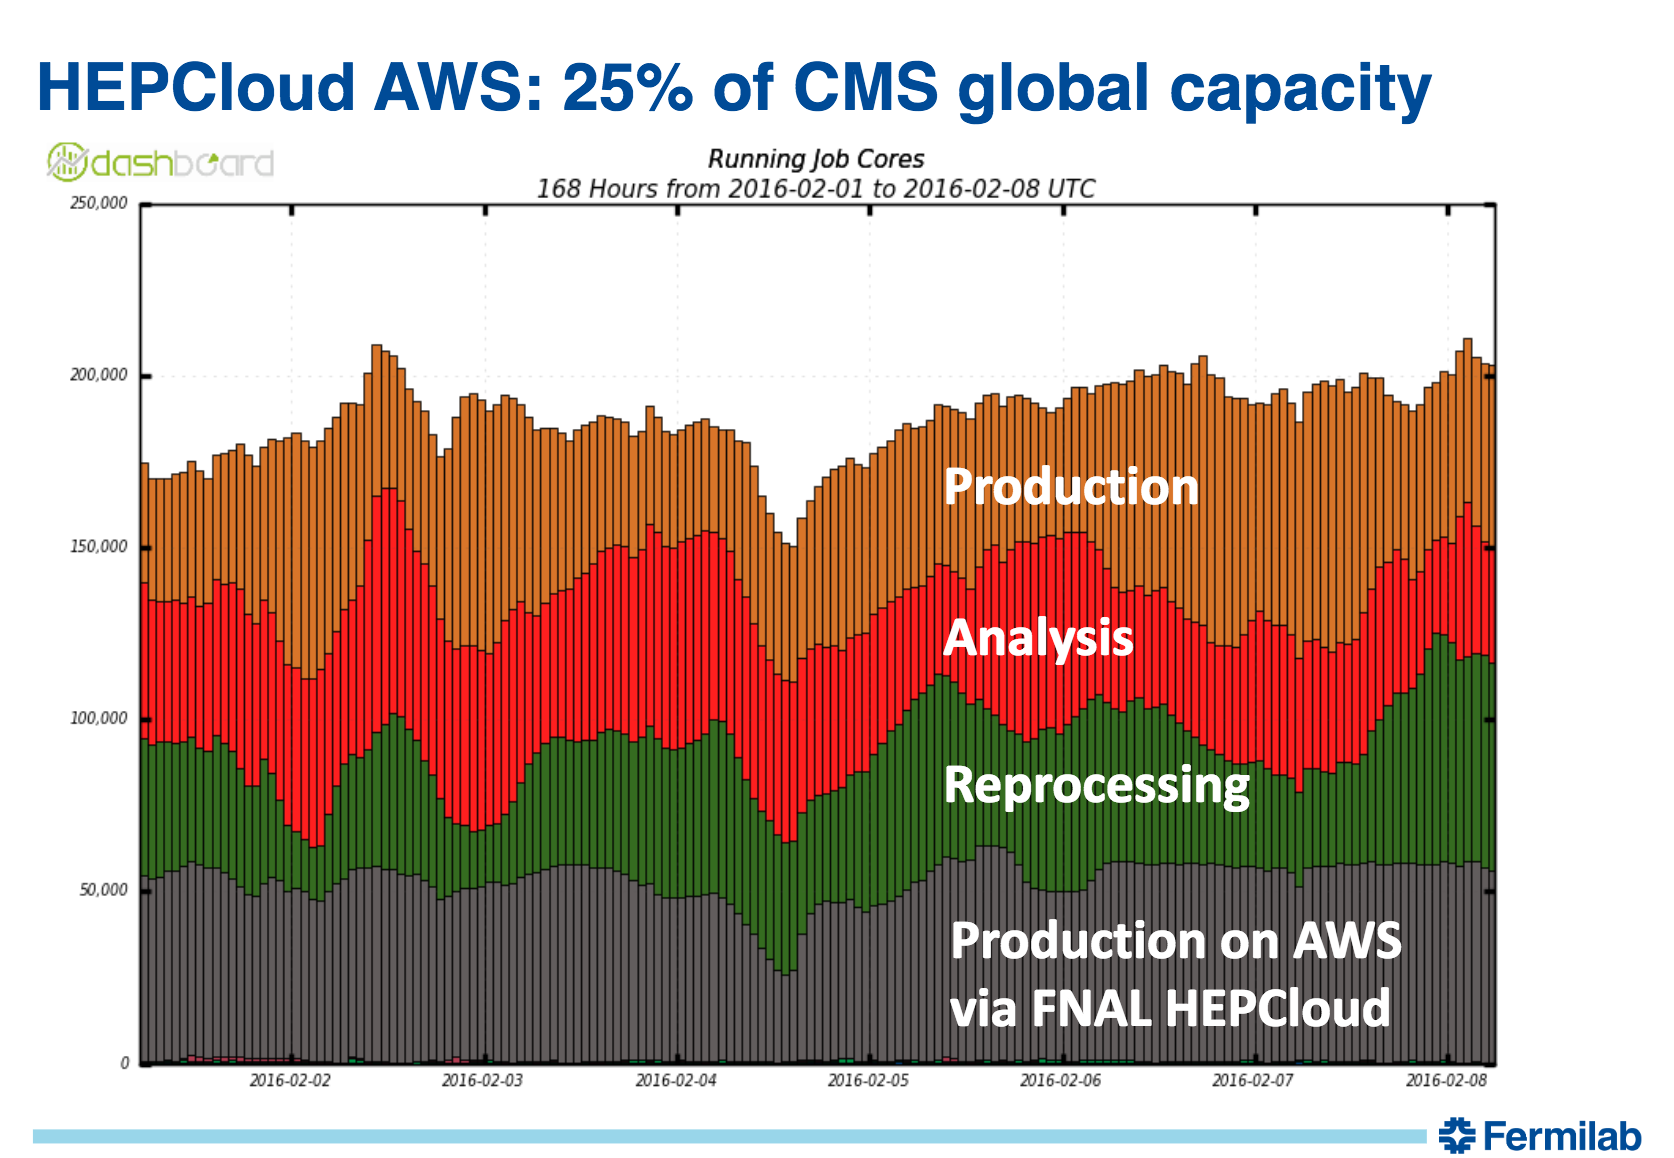
\includegraphics[width=0.7\textwidth]{images/hepcloud-aws.png}
%\caption{}
%\label{fig:example2}
\end{center}
\end{figure}

\end{frame}



\begin{frame}
\frametitle{HepCloud (Fermilab) Google Cloud test}

\begin{figure}[htbp]
\begin{center}
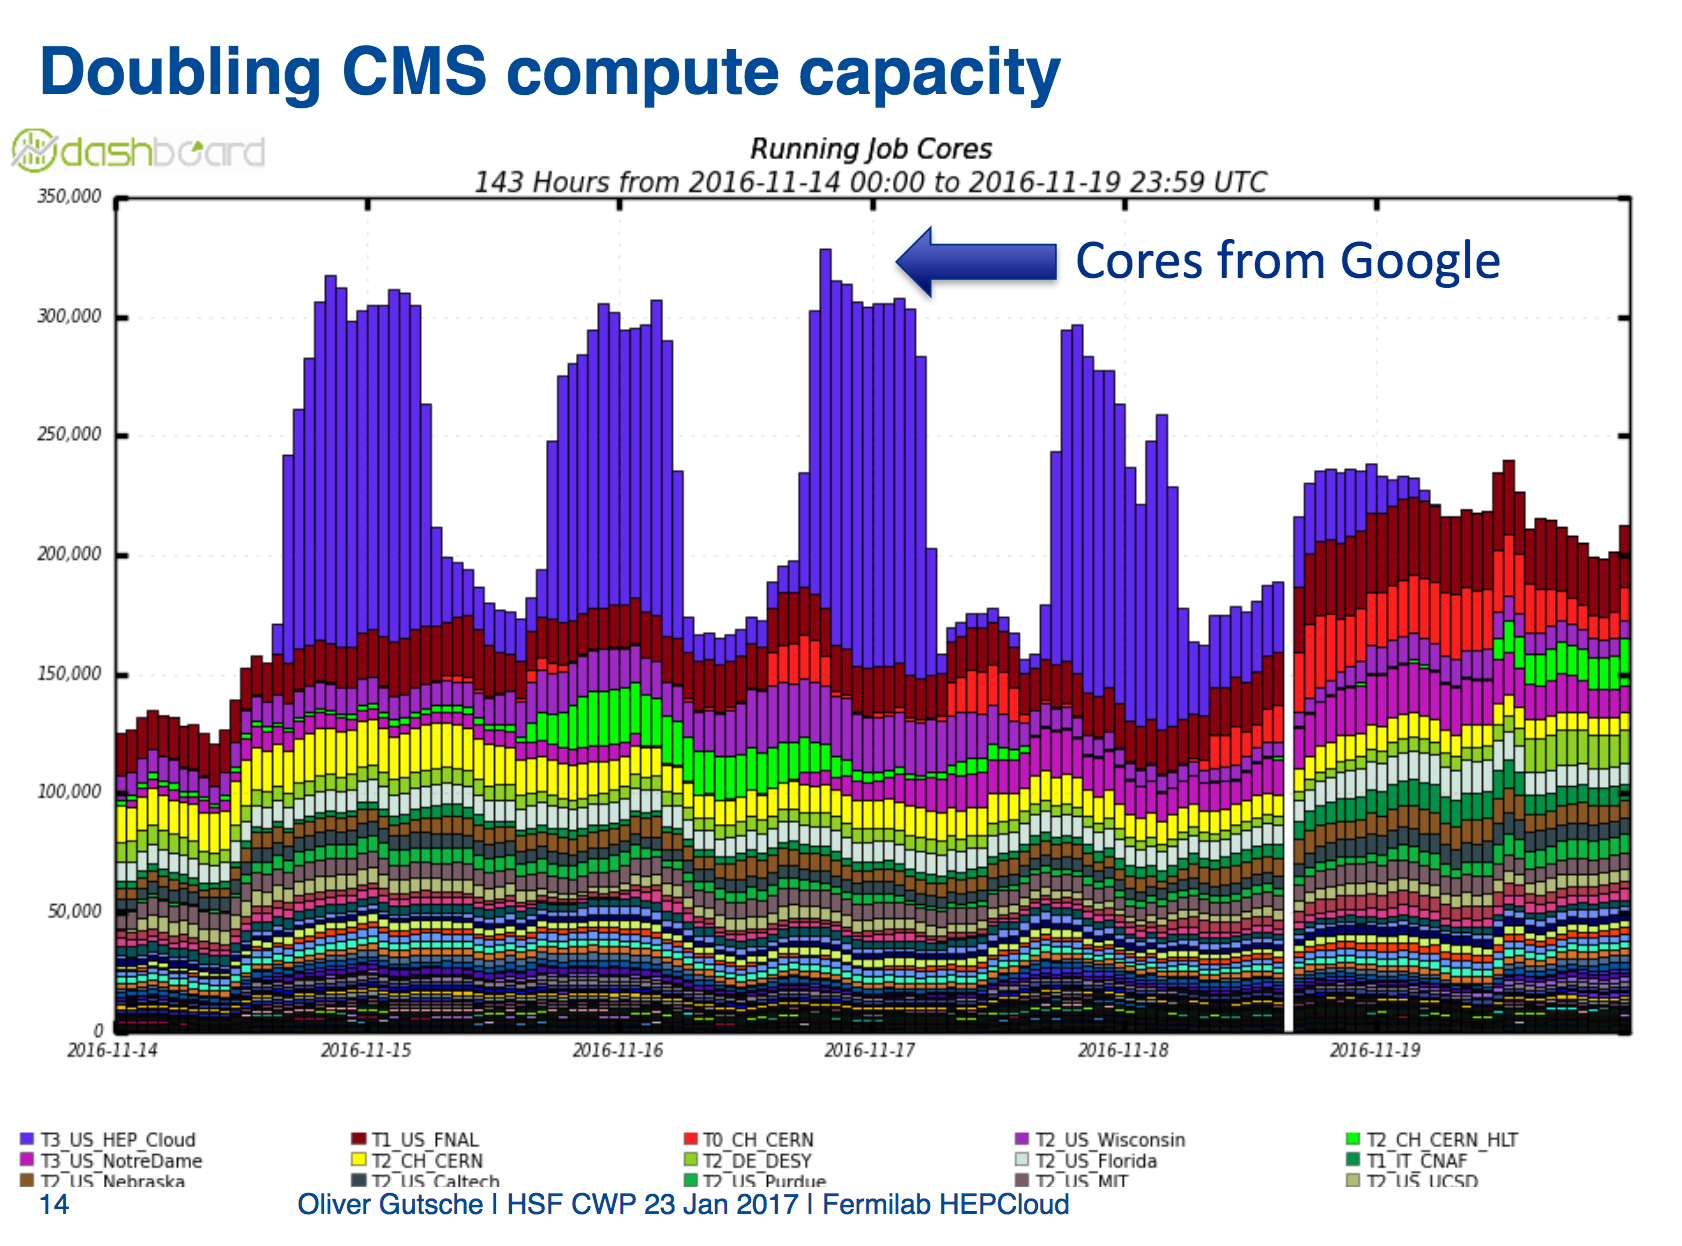
\includegraphics[width=0.7\textwidth]{images/hepcloud-google.png}
%\caption{}
%\label{fig:example2}
\end{center}
\end{figure}

\end{frame}




\end{document}
